\chapter{Introduction}

I introduce a sample of master's thesis \cite{taro}.


\section{Sample}

The followings are samples.
I assume an $n$-dimensional hypersphere shown in Eq. \eqref{eq:eq_1_1}.
In case of $n=3$, the shape is like in Figure \ref{fig:ball 1}.
\begin{align}
	r^2 = \sum_{k=1}^n x_k^2
	\label{eq:eq_1_1}
\end{align}
\begin{figure}[h]
	\centering
	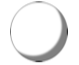
\includegraphics[bb=0 0 79 65]{./figures/ball.png}
	\caption{A sphere where $n=3$}
	\label{fig:ball 1}
\end{figure}

According to Table \ref{table:elem 1}, it has four elements (a,b,c,d).
\begin{table}[h]
	\centering
	\begin{tabular}{|c|c|}
		\hline
		a & b \\ \hline
		c & d \\ \hline
	\end{tabular}
	\caption{Elements}
	\label{table:elem 1}
\end{table}

